
% ++++++++++++++++++++++++++++++++++++++++++++++++++++++++++++++++++++++++
\newpage
\hypertarget{appendix-movies}{}%neu
\section{Movies and Fictional Literature with Relation to Cryptography}
\label{s:appendix-movies}
% {\bf movies and literature related to cryptography}(see appendix \ref{s:appendix-movies})
\index{movies}
\index{literature}


Cryptographic applications -- classical as well as modern ones -- have been
used in literature and movies. In some media they are only mentioned and
are a pure admixture; in others they play a primary role and are explained
in detail; and sometimes the purpose of the story, which forms the framework,
is primarily to transport this knowledge and achieve better motivation.
Here is the beginning of an overview.

% --------------------------------------------------------------------------
\subsection{For Grownups and Teenagers}

\begin{description}

\item[\textrm{[Poe1843]}] \index{Poe 1843}
    Edgar Allan Poe\index{Poe, Edgar Allan}, \\
    {\em The Gold Bug}, 1843. \\
    In this short story Poe tells as first-person narrator about his
    acquaintanceship with the curious Mr. Legrand. They detect a fabulous
    treasure via a gold bug and a vellum found at the coast of New England.\\
    The cipher consists of 203 cryptic symbols and it proves to be a
    general monoalphabetic substitution cipher (see
    chapter~\ref{monoalphabeticSubstitutionCiphers}).
    The story tells how they solve the riddle step by step using a combination
    of semantic and syntax analysis (frequency analysis of single letters in
    English texts).\\
    In this novel the code breaker Legrand says the famous statement:
    ``Yet it may be roundly asserted that human ingenuity cannot concoct a
    cipher which human ingenuity cannot resolve -- given the according
    dedication.''\\
    % Yet it may be roundly asserted that human ingenuity cannot concoct a
    % cipher which human ingenuity cannot resolve...


\item[\textrm{[Verne1885]}] \index{Verne 1885}
    Jules Verne\index{Verne, Jules}, \\
    {\em Mathias Sandorf}, 1885. \\
    This is one of the most famous novels of the French author Jules Verne
    (1828-1905), who was called ``Father of Science fiction''.\\
    In ``Mathias Sandorf'' he tells the story of the freedom fighter Earl
    Sandorf, who is betrayed to the police, but finally he can escape.\\
    The whistle-blowing worked, because his enemies captured and decrypted
    a secret message sent to him. For decryption they needed a special
    grille, which they stole from him. This turning grille was a quadratic
    piece of jig with 6x6 squares, of which 1/4 (nine) were holes
    (see the \hyperlink{turning-grille}{turning grille} in 
    chapter~\ref{introsamplesTranspositionCiphers}).\\


\item[\textrm{[Kipling1901]}] \index{Kipling 1901}
    Rudyard Kipling\index{Kipling, Rudyard}, \\
    {\em Kim}, 1901. \\
    Rob Slade's review%
    \footnote{See
        \url{http://catless.ncl.ac.uk/Risks/24.49.html#subj12}.
    }
    of this novel says:
    ``Kipling packed a great deal of information and concept into his stories,
    and in ``Kim'' we find The Great Game: espionage and spying.  Within the
    first twenty pages we have authentication by something you have, denial
    of service, impersonation, stealth, masquerade, role-based
    authorization (with ad hoc authentication by something you know),
    eavesdropping, and trust based on data integrity.  Later on we get
    contingency planning against theft and cryptography with key changes.''\\
    The book is out of copyright%
    \footnote{You can read it at:\\
          \url{http://whitewolf.newcastle.edu.au/words/authors/K/KiplingRudyard/prose/Kim/index.html},\\
          \url{http://kipling.thefreelibrary.com/Kim} or\\
          \url{http://www.readprint.com/work-935/Rudyard-Kipling}.
    }.\\


\item[\textrm{[Doyle1905]}] \index{Doyle 1905}
    Arthur Conan Doyle\index{Doyle, Sir Arthur Conan}, \\
    {\em The Adventure of the Dancing Men}, 1905. \\
    In this Sherlock Holmes short story (first published in 1903 in the
    ``Strand Magazine'', and then in 1905 in the collection 
    ``The Return of Sherlock Holmes'' the first time in book-form)
    Sherlock Holmes has to solve a cipher which at first glance looks
    like a harmless kid's picture. \\
    But it proves to be the monoalphabetic substitution cipher (see
    chapter~\ref{monoalphabeticSubstitutionCiphers}) of the criminal Abe
    Slaney.
    Sherlock Holmes solves the riddle using frequency analysis.\\


\item[\textrm{[Sayers1932]}] \index{Sayers 1932}
    Dorothy L. Sayers, \\
    {\em Have his carcase}, Harper/Victor Gollancz Ltd., 1932. \\
    In this novel the writer Harriet Vane finds a dead body at the beach.
    The police believe the death is suicide.
    Harriet Vane and the elegant amateur sleuth Lord Peter Wimsey together
    clear of the disgusting murder in this second of Sayers's famous
    Harriet Vane mystery series. \\
    This requires to solve a cryptogram. Surprisingly the novel not only
    describes the Playfair cipher in detail, but also the cryptanalysis
    of this cipher
    (see \hyperlink{playfair}{Playfair} in 
    chapter~\ref{polygraphicSubstitutionCiphers}).\\


\item[\textrm{[Simmel1970]}] \index{Simmel 1970}
    Johannes Mario Simmel, \\
    {\em And Jimmy went to the Rainbow (original title: Und Jimmy ging zum
    Regenbogen)}, Knaur Verlag, 1970. \\
    The novel plays between 19938 and 1967 in Vienna. The main character Manual
    Aranda uncovers step by step the past of his murdered father. Important for
    the plot is an encrypted manuscript, which is decrypted in chapter 33. In
    the novel the cipher is called ``25-fold Caesar cipher''. It is actually a
    Vigen\`ere cipher with a 25 character key.\\
    A movie of the novel appeared in 1971.\\


\item[\textrm{[Crichton1987]}] \index{Crichton 1987}
    Michael Crichton, \\
    {\em Sphere}, Pan Books, 1987. \\
    A team of different scientists is send to the ground of the ocean in order to
    investigate a highly developed 900~m long space ship. The human peculiarities 
    and psychological problems of the researchers surface more and more, because of 
    life threatening events and isolation. There are many mysteries: While the
    space ship lies on the ground for 300 years, it has English markings and a life
    of its own, and materializing of the researcher's imaginations appear. On a
    computer screen a cipher text appears, which is completely printed in the book.
    The genius mathematician Harry deciphers the simple helical substitution code.\\

\item[\textrm{[Seed1990]}] \index{Seed 1990}
    Directed by Paul Seed, \\
    {\em House of Cards}, 1990. \\
    In this movie Ruth tries to solve the secret, which made her daughter
    fall silent. Here two young people suffering from autism communicate
    via 5- and 6-digit primes (see 
    chapter~\ref{Label_Kapitel_Primes}).
    After more than 1 hour the movie contains the following encrypted
    two series of primes:
    \begin{center}
    $21,383; \;\;176,081; \;\;18,199; \;\;113,933; \;\;150,377; \;\;304,523; \;\;113,933$ \\
    $193,877; \;\;737,683; \;\;117,881; \;\;193,877$
    \end{center}
    % where autistic children communicate via primes
    \vskip +20 pt


\item[\textrm{[Robinson1992]}] \index{Robinson 1992}
    Directed by Phil Alden Robinson, \\
    {\em Sneakers}, Universal Pictures Film, 1992. \\
    In this movie the ``sneakers'', computer experts under their boss Martin
    Bishop, try to get back the deciphering box SETEC from the ``bad guys''.
    SETEC, invented by a genius mathematician before he was killed, allows to
    decrypt all codes from any nation. \\
    In the movie the code is not described in any way%
    \footnote{
       Leonard Adleman (the "A" within RSA) worked as mathematical consultant
       for ``Sneakers''. He describes the funny story about his contribution
       at his homepage 
       \url{http://www.usc.edu/dept/molecular-science/fm-sneakers.htm}.
       It is assumed that the cipher used everywhere is RSA.      
       According to that within the chip a fast, unknown factorization
       method\index{factorization} is implemented.
    }.\\


\item[\textrm{[Baldacci1997]}] \index{Baldacci 1997}
    David Baldacci, \\
    {\em Total Control}, Mass Market Paperback, 1997. \\
    Jason Archer, executive with a technology company suddenly disappears.
    Sidney Archer tries to find out about her husband's surprising death.
    She gets a clue how the global financial system is abused and that the
    real control belongs to those with the most money. Here even good passwords
    don't help ...\\


\item[\textrm{[Natali1997]}] \index{Natali 1997}
    Directed by Vincenzo Natali, \\
    {\em Cube}, Mehra Meh Film, 1997. \\
    In this Canadian low-budget-movie 7 complete strangers of widely varying
    personality characteristics are involuntarily placed in an kafkaesque maze
    of cubical rooms containing deadly traps.\\
    To get out the persons have to move through these rooms. To find out
    which rooms are dangerous, mathematics is crucial: Each cubic room has
    at its entrance a numerical marking consisting of three sets of three
    digits. First they deduce that all rooms marked at their entrance with
    at least one prime number are trapped. Later it comes out that a trapped
    room can also be marked by a number which is a power of a prime (so 
    traps are $p^n$, e.g. $128=2^7$ or $101 = 101^1 = prime$, but not
    $517 = 11*47$).\\


\item[\textrm{[Becker1998]}] \index{Becker 1998}
    Directed by Harold Becker, \\
    {\em Mercury Rising}, Universal Pictures Film, 1998. \\
    The NSA developed a new cipher, which is pretended to be uncrackable by
    humans and computers. To test its reliability some programmers hide a
    message encrypted with this cipher in a puzzle magazine.\\
    Simon, a nine year old autistic boy, cracks the code. Instead of
    fixing the code, a government agent sends a killer. FBI agent Art
    Jeffries (Bruce Willis) protects the boy and sets a snare for the
    killers.\\    
    The code is not described in any way.\\


\item[\textrm{[Brown1998]}] \index{Brown 1998}
    Dan Brown, \\
    {\em Digital Fortress}, E-Book, 1998. \\
    Dan Brown's first novel was published in 1998 as e-book, but it was
    largely unsuccessful then.\\
    The National Security Agency (NSA) uses a huge computer, which enables it
    to decrypt all messages (needless to say only of criminals and terrorists)
    within minutes even if they use the most modern encryption methods.\\
    An apostate employee invents an unbreakable code and his computer program
    Diabolus forces the super computer to do self destructing operations.
    The plot, where also the beautiful computer expert Susan Fletcher has a
    role, is rather predictable.\\
    The idea, that the NSA or another secret service is able to decrypt any
    code, is currently popular on several authors: In ``Digital Fortress'' the
    super computer has 3 million processors -- nevertheless from today's sight
    this is by no means sufficient to hack modern ciphers.\\


\item[\textrm{[Elsner1999]}] \index{Elsner 1999}
    Dr.~C.~Elsner, \\
    {\em The Dialogue of the Sisters}, c't, Heise, 1999. \\
    In this short story, which is included in the CrypTool package
    \index{CrypTool} as PDF file, the sisters confidentially communicate
    using a variant of RSA (see chapter~\ref{rsabeweis} and the following).
    They are residents of a madhouse being under permanent surveillance.\\


\item[\textrm{[Stephenson1999]}] \index{Stephenson 1999}
    Neal Stephenson, \\
    {\em Cryptonomicon}, Harper, 1999. \\
    This very thick novel deals with cryptography both in WW2 and today.
    The two heroes from the 40ies are the excellent mathematician and
    cryptanalyst Lawrence Waterhouse, and the overeager and 
    morphine addicted US marine Bobby Shaftoe. 
    They both are members of the special allied unit 2702, which tries
    to hack the enemy's communication codes and at the same time to
    hide the own existence. \\
    This secretiveness also happens in the present plot, where the 
    grandchildren of the war heroes -- the dedicated programmer  
    Randy Waterhouse and the beautiful Amy Shaftoe -- team up. \\
    Cryptonomicon is notably heavy for non-technical readers in parts.
    Several pages are spent explaining in detail some of the concepts
    behind cryptography.
    Stephenson added a detailed description of the Solitaire cipher
    (see chapter~\ref{Further-PaP-methods}), a paper and pencil encryption
    algorithm\index{paper and pencil methods} developed by Bruce Schneier
    which is called ``Pontifex'' in the book. Another, modern algorithm
    called ``Arethusa'' is not explained in detail.\\


\item[\textrm{[Elsner2001]}] \index{Elsner 2001}
    Dr.~C.~Elsner, \\
    {\em The Chinese Labyrinth}, c't, Heise, 2001. \\
    In this short story, which is included in the CrypTool package
    \index{CrypTool} as PDF file, Marco Polo has to solve problems from
    number theory within a competition to become a major consultant of
    the Great Khan. All solutions are included and explained.\\


\item[\textrm{[Colfer2001]}] \index{Colfer 2001}
    Eoin Colfer, \\
    {\em Artemis Fowl}, Viking, 2001. \\
    In this book for young people the 12 year old Artemis, a genius thief,
    gets a copy of the top secret ``Book of the Elfs''. After he decrypted it
    with his computer, he finds out things, men never should have known. \\
    The used code is not described in detail or revealed.\\


\item[\textrm{[Howard2001]}] \index{Howard 2001}
    Directed Ron Howard, \\
    {\em A Beautiful Mind}, 2001. \\
    This is the film version of Sylvia Nasar's biography of the game theorist
    John Nash. 
    After the brilliant but asocial mathematician accepts secret work in 
    cryptography, his life takes a turn to the nightmarish.
    His irresistible urge to solve problems becomes a danger for himself and
    his family. Nash is -- within his belief -- a most important hacker
    working for the government.\\
    Details of his way analysing code are not described in any way.\\


\item[\textrm{[Apted2001]}] \index{Apted 2001}
    Directed by Michael Apted, \\
    {\em Enigma}, 2001. \\
    This is the film version of Robert Harris' ``historical fiction'' 
    {\em Enigma} (Hutchinson, London, 1995) about the World War II 
    code-breaking work at Bletchley Park in early 1943, when the actual
    inventor of the analysis Alan Turing (after Polish pre-work) already 
    was in the US.
    So the fictional mathematician Tom Jericho is the lead character
    in this spy-thriller.\\
    Details of his way analysing the code are not described.\\


\item[\textrm{[Isau2003]}] \index{Isau 1997}
    Ralf Isau, \\
    {\em The Museum of the stolen memories (original title: Das Museum
    der gestohlenen Erinnerungen)}, Thienemann-Verlag, 1997/2003. \\
    In this exciting novel the last part of the oracle can only be
    solved with the joined help of the computer community.\\
    The book got several awards and exists in 8 different languages,
    but not in English yet.\\


\item[\textrm{[Brown2003]}] \index{Brown 2003}
    Dan Brown, \\
    {\em The Da Vinci Code}, Doubleday, 2003. \\
    The director of the Louvre is found murdered in his museum in
    front of a picture of Leonardo da Vinci. And the symbol researcher
    Robert Langdon is involved in a conspiracy.
    The plot mentions different classic codes (substitution like
    Caesar or Vigen\`ere, as well as transposition and number codes).
    Also there are hints about Schneier and the sunflower.
    The second part of the book contains a lot of theological considerations.\\
    This book has become one of the most widely read books of all time.\\


\item[\textrm{[Hill2003]}] \index{Hill 2003}
    Tobias Hill, \\
    {\em The Cryptographer}, Faber \& Faber, 2003. \\
    London 2021: The company SoftMark developed and establish an electronic
    curreny, which guarantees highest security standards by an unbreakable code.
    The inventor and company founder, called the cryptographer because of his
    mathematical talent, has become the richest man in the world.
    But the code was hacked, and in a worldwide economic crisis his company
    goes bankrupt.
    Additionally the tax investigator Anna Moore is set on him.\\


\item[\textrm{[McBain2004]}] \index{McBain 2004}
    Scott McBain, \\
    {\em Final Solution}, manuscript not published by Harper Collins, 2004
    (German version has been published in 2005). \\
    In a near future politicians, chiefs of military and secret services of
    many different countries take over all the power. With a giant computer
    network called ``Mother'' and complete surveillance they want to cement
    their power and commercialisation of life forever.
    Humans are only assessed according to their credit rating and globally
    acting companies elude of any democratic control.
    Within the thriller the obvious injustice, but also the realistic
    likelihood of this development are considered again and again.\\
    With the help of a cryptographer a code to destroy was built into the
    super computer ``Mother'': In a race several people try to start the
    deactivation (Lars Pedersen, Oswald Plevy, the female American president,
    the British prime minister and an unknown Finish named Pia, who wants to
    take revenge for the death of her brother). On the opposite side a killing
    group acts under the special guidance of the British foreign minister and
    the boss of the CIA.\\


\item[\textrm{[Preston2005]}] \index{Preston 2005}
    Douglas Preston, \\
    {\em Tyrannosaur Canyon}, Forge Books, 2005. \\
    A very exciting thriller which also struggles with the question why the dinosaurs
    died off.

    Archeologist Stem Weathers is shot in a canyon. Before his murderer appears he
    gives his notebook to Tom Broadbent, a local animal doctor, coming by accidentally.
   
    The notebook contains on 60 pages only digits. Therefore Tom takes it to Wyman Ford
    an ex-CIA cryptanalyst, who now lives in a nearby abbey, after his wife was killed
    in action.
    Wyman first declines and says that self-invented code are ``idiot ciphers'' -- devised
    by an idiot and easily crackable by each idiot. The notebook then proves to be not
    that easy. After intensive analysis he finds out that the digits are no code but the
    output of an earth radar device showing the picture of a well-preserved T.rex.

    After around 250 pages of endless chases a surprising turn comes up: Masago, head
    of a so-called black-detachment unit of the CIA. He explains: New weapons
    invented once always have been used. Mankind will kill herself, but its his task
    to postpone that as far as possible. As head of the LS480 department he will prevent
    by any means possible that terrorists get any new dangerous biological weapon.

    When scanning the dead body of Weathers the murder only found some rock cuttings
    he took. These rocks are investigated by a young reseacher named Melody Crookshank
    although she doesn't know where the rock cuttings come from. She finds within
    them a very special kind of virus  apparently coming from outer-space.\\



\item[\textrm{[Burger2006]}] \index{Burger 2006}
    Wolfgang Burger, \\
    {\em Heidelberg Lies (original title: Heidelberger L\"ugen)}, Piper, 2006. \\
    This detective story playing in the Rhein-Neckar area in Germany has
    several independent strands and local stories, but mainly it is
    about Kriminalrat Gerlach from Heidelberg. On page 207 f. the
    cryptographic reference for one strand is shortly explained: The
    soldier H\"orrle had copied circuit diagrams of a new digital NATO
    decryption device and the murdered man had tried to sell his perceptions
    to China.\\



\item[\textrm{[Twinig2006]}] \index{Twinig 2006}
    James Twinig, \\
    {\em The Black Sun}, HarperCollins, 2006. \\
    A history-based thriller with some artificially constructed elements, dealing
    also with a treasure hunt to get the hidden uranium of the nazis, and
    naturally the future of the world depends on today's bad guys being stopped in time ...

    Heros are Tom Kirk, a London-based ex-CIA agent and former professional art thief,
    and Dominique de Lecourt, who loves challenges including riddles and codes.

    The only cryptographic parts are a ``Sprungcode'' (the criminals use this method to
    communicate via newsletter adverts), steganography (used to hide the Enigma key),
    and an Enigma message (containing the encrypted coordinates of the treasure).

    At the beginning of the plot an Enigma device is stolen with high efforts
    which is necessary to let the story play in the constructed way. But in the
    reality today such a theft is completely needless, as there are great software
    emulators for the Enigma ... \\



\item[\textrm{[Vidal2006]}] \index{Vidal 2006}
    Agustin Sanchez Vidal, \\
    {\em Kryptum}, Dtv, 2006. \\
    The first novel of the Spanish professor of art history has some
    similarities with Dan Brown's ``The Da Vinci Code'' from 2003, but allegedly
    Vidal started his writing of the novel already in 1996. Vidal's novel is
    a mixture between historic adventure and mystery thriller.
    It was a huge success in Spain and Germany.
    There is currently no English version available.\\
    In the year 1582 Raimundo Randa is waiting to be condemned to death -- he
    was all life long trying to solve a mystery.
    This mystery is about a parchment with cryptic characters, where a unique
    power is behind.
    Around 400 years later the American scientist Sara Toledano is fascinated
    by this power until she vanishes in Antigua.
    Her colleague, the cryptographer David Calderon, and her daughter Rachel
    are searching for her and simultaneously they try to solve the code.
    But also secret organizations like the NSA chase after the secret
    of the ``last key''. They don't hesitate to kill for it.\\


\item[\textrm{[Larsson2006]}] \index{Larsson 2006}
    Stieg Larsson, \\
    {\em Perdition (original title: Flickan som lekte med elden)}, 2006. \\
    The author was posthumously awarded in 2006 with the Scandinavian thriller 
    award. The super hero Lisbeth Salander uses PGP and occupies herself 
    with mathematical riddles like the Fermat theorem.\\


\item[\textrm{[Schroeder2008]}] \index{Schroeder 2008}
    Rainer M. Schr\"oder, \\
    {\em The Judas Documents (original title: Die Judas-Papiere)}, Arena, 2008. \\
    In the year 1899 Lord Pembroke has three men and one woman in his grip.
    So they have to follow his order to try to decipher the encrypted messages
    in the notebook of his dead brother Mortimer and to find the missing gospel
    according to Judas, which could shock the whole of Christendom. The four
    people therefor have to solve riddles at many places in the world.
    The story explains some classic ciphers like Polybius and Freemason.\\


\item[\textrm{[Eschbach2009]}] \index{Eschbach 2009}
    Andreas Eschbach, \\
    {\em A King for Germany (original title: Ein K\"onig f\"ur Deutschland)},
    L\"ubbe, 2009.\\
    The novel deals with manipulations of electronic voting machines.\\
    Vincent Merrit, a young US-American programmer, is blackmailed,
    to write such a programme. Beside commercially oriented blackmailers
    also Massively Multiplayer Online Role-Playing Games (MMORPGs) and
    Live Action Role Playing (LARP) have a role.
    Because Merrit assumed that his programme will be misused, he installed a
    trapdoor: If a party with the name VWM participates at the election,
    it automatically gets 95 \% of the votes ...\\
    The fictional story line is based on many verifiable and well researched
    facts, which are referenced in footnotes.\\
    While the cryptographic protocols itself could be made secure,
    their implementation and their organisational management stays susceptible
    against misuse.\\
    Currently there is no English translation of the book.\\


\item[\textrm{[Juels2009]}] \index{Juels 2009}
    Ari Juels, \\
    {\em Tetraktys}, Emerald Bay Books, 2009.\\
    The plot exposes the vulnerability of modern computer based identity, authenticity,
    and security interweaving modern cryptography with classical art and literature.
    Cryptographer and classicist Ambrose Jerusalem is a UC Berkeley graduate
    with a beautiful girlfriend and a comfortable future, until the NSA recruits him
    to track a strange pattern of computer break-ins. Many small pieces provide
    disturbing evidence that someone has broken RSA encryption. Even more bizarre,
    a secret cult of latter-day followers of Pythagoras, the great Greek mathematician
    and philosopher who believed reality could be understood only through a mystical
    system of numbers, appears to be behind the attacks.\\


\item[\textrm{[Suarez2009]}] \index{Suarez 2009}
    Daniel Suarez, \\
    {\em Daemon}, Penguin Books, 2009, 632 pages. \\
    This is considered as one of the most exciting books during the last few years -- its a
    near-science-fiction thriller combining developments in the real world and possibilities
    coming from current research like from the Google X Lab (augmented reality
    head-mounted displays (HMD) like Google glass, self-driving cars, 3-D printers, ...)
    to a plausible story.

    After the computer genius and game developer Matthew Sobol died a daemon starts
    acting in the internet, which seemingly ruthless manipulates and trains more and more
    humans and companies.

    By ruling the data everybody seems to be a helpless victim. All the communication
    of his mercenary soldiers is affected by high-tech and encryption -- also the
    communication between the distributed instances of his incarnation. Core is an MMORPG
    game (massive multiplayer online role-playing game) which reminds many of WoW. Here also
    encryption is used, e.g. to advertise the best players: m0wFG3PRCoJVTs7JcgBwsOXb3U7yPxBB

    The plot is without redudancy, complex, manifold, very fascinating and with it
    critics about the plutocrats it also contains concrete social elements.
    The end is open. And the ideas seem to be realizable in the very next future ...\\


\item[\textrm{[Suarez2010]}] \index{Suarez 2010}
    Daniel Suarez, \\
    {\em Freedom (TM)}, Penguin Books, 2010, 486 pages. \\
    ``The propulsive, shockingly plausible sequel to the bestseller Daemon'' (see above).
    Freedom (TM) (Daemon \#2) patches a number of holes the writer left in the first book.
    The prose is tighter, the descriptions more direct, the characters are fleshed out,
    especially Loki.
    Having laid the groundwork in ``Daemon'', Suarez uses this
    foundation in order to explore a new concept of social organization based on empowering
    information technology and the reasoning why and how the battle runs between the old
    potentates and the Daemon society, which also evolves further already during the story.
    Cryptography is a natural part of modern technology and modern warfare as described
    in this book.
    The new society emerging in "Freedom (TM)" is based on the darknet, an alternative to
    the internet using fast wireless meshes in order to increase the durability and
    availability of the network. Despite the story is shocking in some parts, it appears to
    be realistic and not far away from the parallel usage of modern technology integrated
    into our modern lives as a virtual world overlaying our real world.\\


\item[\textrm{[Burger2011]}] \index{Burger 2011}
    Wolfgang Burger, \\
    {\em The fifth murderer (original title: Der f\"unfte M\"order)}, Piper, 2011. \\
    Location \& time of the story: Germany / Heidelberg, 1990 - 2009. 
    Episode 7 of the Alexander-Gerlach series.
    Inspector Alexander Gerlach became almost a victim of a bomb blast when the
    sport utility vehicle (SUV) of a Bulgarian panderer exploded.
    Gerlach starts investigating because he wants to prevent a gang warfare, but then
    his bosses call him off.
    When the journalist Machatschek supports Gerlach, he communicates with him only via
    Skype using an add-on encryption program which he believes is the most secure in the
    world.\\



\item[\textrm{[Elsberg2012]}] \index{Elsberg 2012}
    Marc Elsberg, \\
    {\em Blackout -- Tomorrow its too late (original title: Blackout -- Morgen ist
    es zu sp\"at)},\\ Blanvalet, 2012, 800 pages. \\
    At a could day in winter all power supply networks in Europe break down.
    Agencies, energy suppliers and security companies are in the dark and unable to solve
    the problem.
    The Italian computer scientist Piero Manzano believes that this caused by terrorists
    using hackers: All customers use since some years smart meters, electricity meters
    controlled by software which was manipulated. Despite the integrated security and encryption
    components they have been hacked, and are out of order by wrong control sequences.
    The terrifying consequences at various locations are described realistically and excitingly.
    And in the same way the reactions of the human beings ...\\


\end{description}



\vskip +20 pt
\paragraph*{Remark 1:}
Further samples of cryptology in fictional literature can be found on the
following German web page:
\parskip -4pt  % 1-BACK to DEFAULT -- Really necessary
\begin{center}
    \url{http://www.staff.uni-mainz.de/pommeren/Kryptologie99/Klassisch/1\_Monoalph/Literat.html}
\end{center}
\parskip \value{mycounterDefaultParskip} pt  % 2-BACK to DEFAULT -- Really necessary
For some older authors (e.g. Jules Verne, Karl May, Arthur Conan Doyle,
Edgar Allen Poe) there are links to the original and relevant text pieces.\\


\paragraph*{Remark 2:}
You can find title pages of some of these books on the web site of
Tobias Schr\"odel\index{Schroedel, Tobias}, who collects classic books about cryptography:
\parskip -4pt  % 1-BACK to DEFAULT -- Really necessary
\begin{center}
   \url{http://tobiasschroedel.com/crypto_books.php}
\end{center}
\parskip \value{mycounterDefaultParskip} pt  % 2-BACK to DEFAULT -- Really necessary
\vspace{1em}


\paragraph*{Remark 3:}
If you know of further books and movies, where cryptography has a major
role then we would be very glad if you could send us the exact title and
a short explanation about the movie/book's content. Thanks a lot.\\






% --------------------------------------------------------------------------
\newpage
\subsection{For Kids and Teenagers}

The following list contains movies and ``kid books''.
The kid books contain both stories, and collections of simple ciphers, prepared
in a didactic and exciting manner
(please send us similar English kid books and kid movies, because at the moment
our list contains mostly German kid books):

\begin{description}

\item[\textrm{[Mosesxxxx]}] \index{Moses xxxx}
    [no named author], \\
    {\em Top secret -- The Book for Detectives and Spies (original title:
    Streng geheim -- Das Buch f\"ur Detektive und Agenten)},
    Edition moses, [no year named]. \\
    This is a thin book for small kids with Inspector Fox and Dr. Chicken.\\


\item[\textrm{[Arthur196x]}] \index{Arthur 196x}
    Robert Arthur, \\
    {\em The Three Investigators: The Secret Key (German version:  Die 3 ???: Der
    geheime Schl\"ussel nach Alfred Hitchcock (volume 119)},
    Kosmos-Verlag (from 1960) \\
    The three detectives Justus, Peter and Bob have to decrypt covered and
    encrypted messages within this story to find out what is behind the toys
    of the Copperfield company.\\


\item[\textrm{[Para1988]}] \index{Para 1988}
    Para, \\
    {\em Ciphers (original title: Geheimschriften)},
    Ravensburger Taschenbuch Verlag, 1988 (1st edition 1977). \\
    On 125 pages filled with a small font this mini format book explains
    many methods which young children can apply directly to encrypt or hide
    their messages. A little glossary and a short overview about the usage of
    encryption methods in history complete this little book.

    Right at page 6 it summarizes for beginners in an old fashion style
    ``The Important Things First'' about paper\&pencil encryption
    (compare chapter~\ref{Kapitel_PaperandPencil}):
    \begin{itemize}
      \item[-] ``It must be possible to encrypt your messages at any place and
               at any location with the easiest measures and a small effort
               in a short time.
      \item[-] Your cipher must be easy to remember and easy to read for your
               partners. But strangers should not be able to decrypt them.\\
               Remember: Fastness before finesse, security before carelessness.
      \item[-] Your message must always be as short and precise as a telegram.
               Shortness outranks grammar and spelling. Get rid of all needless
               like salutations or punctuation marks. Preferably use only
               small or only capital letters.''
    \end{itemize}
    \vskip +20 pt   % da "\\" hier nicht geht!


\item[\textrm{[M\"uller-Michaelis2002]}] \index{M\"uller-Michaelis 2002}
    Matthias M\"uller-Michaelis, \\
    {\em The manual for detectives. Everything you need to know about
     ciphers, codes, reading tracks and the biggest detectives of the world
     (original title: Das Handbuch f\"ur Detektive. Alles \"uber
     Geheimsprachen, Codes, Spurenlesen und die gro\ss en Detektive dieser
     Welt)}, S\"udwest, 2002. \\


\item[\textrm{[Kippenhahn2002]}] \index{Kippenhahn 2002}
    Rudolf Kippenhahn, \\
    {\em Top secret! -- How to encrypt messages and to hack codes (original
    title: Streng geheim! -- Wie man Botschaften verschl\"usselt und 
    Zahlencodes knackt)}, rororo, 2002. \\
    In this novel a grandpa, an expert for secret writings teaches his
    four grandchildren and their friends, how to encrypt messages which
    nobody should read. Because there is someone who hacks their secrets,
    the grandpa has to teach them more and more complicated methods. \\
    Within this story, which forms the framework, the most important classic
    encryption methods and its analysis are explained in a manner exciting
    and appropriate for children.\\


\item[\textrm{[Harder2003]}] \index{Harder 2003}
    Corinna Harder and Jens Schumacher, \\
    {\em Top secret. The big book for detectives (original title: 
     Streng geheim. Das gro\ss e Buch der Detektive)}, Moses, 2003. \\


\item[\textrm{[Talke-Baisch2003]}] \index{Talke-Baisch 2003}
    Helga Talke and Milena Baisch, \\
    {\em Your mission in the weird villa. Riddle thriller (original title: 
    Dein Auftrag in der unheimlichen Villa. Kennwort R\"atselkrimi)},
    Loewe, 2003. \\
    From 4th form, ~~~\url{http://www.antolin.de}\\
%    \url{http://www.antolin.de/all/bookdetail.jsp;jsessionid=abcexNCPR6tzlcM5FZpDs?book_id=16224}\\
    Young detectives are faced simple ciphers and codes during their missions.\\



\item[\textrm{[Flessner2004]}] \index{Flessner 2004}
    Bernd Flessner, \\
    {\em The Three Investigators: Manual for Secret Messages (original
    title: Die 3 ???: Handbuch Geheimbotschaften)},
    Kosmos, 2004. \\
    On 127 pages you learn in an easy and exciting manner, structured by
    the method types, which secret languages (like the one of the Navajo
    Indians or dialects) and which secret writings (real encryption or
    hiding via technical or linguistic steganography) existed and how simple
    methods can be decrypted.\\
    The author tells where in history the methods were used and in which
    novel authors used encryption methods [like in Edgar Allan Poe's
    ``The Gold Bug'', like with Jules Verne's hero Mathias Sandorf or like
    with Astrid Lindgren's master detective Blomquist who used the ROR language
    (similar inserting ciphers are the spoon or the B language)].\\
    This is a didactically excellent introduction for younger teens.\\


\item[\textrm{[Z\"ubert2005]}] \index{Z\"ubert 2005}
    Directed by Christian Z\"ubert, \\
    {\em The Treasure of the White Hawks (original title: Der Schatz der 
    wei\ss{}en Falken) }, 2005. \\
    This exciting adventure movie for kids ties in with the tradition of
    classics like ``Tom Sawyer and Huckleberry Finn'' or Enid Blytons
    ``Five Friendse''. The plot happens in summer 1981.
    In an old half tumbledown villa three young kids find the treasure map
    of the ``White Hawks'', which they decrypt with the help of a computer.
    Traced by another gang they aim to go to an old castle.\\


\item[\textrm{[Dittert2011]}] \index{Dittert 2011}
    Christoph Dittert, \\
    {\em The Three Investigators: Secret Messages (German version:  Die 3 ???:
    Geheimnisvolle Botschaften) (volume 160)},
    Kosmos, 2011 \\
    In the house of Professor Mathewson an old hand-made book was stolen.
    The three detectives Justus, Peter and Bob are getting attacked by a ruthless
    opponent, who seems to be always a step ahead.
    A major part in this story is played by a palimpsest, an ancient manuscript page,
    written upon newly. Using X-rays they can make visible again the old text below.
    Its not only the story which is exciting, but also the way, how the instruction for a
    treasure hunt is encrypted. Despite using the simple railfence cipher it's not
    easy to solve it, as the message is distributed onto two slips and as the printed
    symbols don't mean single letters.\\



\end{description}


\vskip +20 pt
\paragraph*{Remark 1:}
You can find title pages of many of these kid books on the web site of
Tobias Schr\"odel\index{Schroedel, Tobias}, who collects classic books about cryptography:
\parskip -4pt  % 1-BACK to DEFAULT -- Really necessary
\begin{center}
   \url{http://tobiasschroedel.com/crypto_books.php}
\end{center}
\parskip \value{mycounterDefaultParskip} pt  % 2-BACK to DEFAULT -- Really necessary
\vspace{1em}


\paragraph*{Remark 2:}
If you know of further books, which address cryptography in a
didactic and for children adequate way, then we would be very glad if
you could send us the exact book title and a short explanation
about the book's content. Thanks a lot.\\






% ++++++++++++++++++++++++++++++++++++++++++++++++++++++++++++++++++++++++++
\newpage
\hypertarget{appendix-Learn-NT}{}
\section{Learning Tool for Elementary Number Theory}
    \label{s:appendix-Learn-NT}  
    \index{NT, Learning Tool for Number Theory}%
    \index{educational tool NT}%

CT1\index{CrypTool 1} contains an interactive educational tool for elementary
{\em number theory}, called ``NT''.\footnote{%
    NT can be called in CT1\index{CrypTool 1} via the menu path
    {\bf Indiv. Procedures \textbackslash{} Number Theory Interactive
    \textbackslash{} Learning Tool for Number Theory}.
}

The educational tool ``NT'' (number theory) by Martin Ramberger introduces
number theory and visualizes many of the methods and concepts.
Where necessary it show the according mathematical formulas.
Often you can apply the mathematical methods dynamically with your own small
numerical examples.

The content of this educational tool is mainly based on the books by J.\ Buchmann and H.\ Scheid
\cite{a:Buchmann2004,a:Scheid2003}.

This visualized educational tool was build with Authorware 4.\footnote{%
    As Authorware is outdated and as the vendor didn't make tools available
    to easily port it to his successor products, the program ZT will not be
    further developed.
}


\paragraph*{Request for enhancement/upgrade:}
It would be desirable to update it to a new version Authorware or to use
another development platform. If there are developers interested to do
this, I'd be more than happy (please send an email at the author of this
CrypTool script).

\paragraph*{Figures:}
The figures~\ref{NT_Fig_C1.3_EuclidsAlg-LinearCombinations}
till~\ref{NT_Fig_C5.3_PollardRho} give you an impression of the
educational tool ``NT'':


% -> Figur 1  WIE ERREICHT MAN, dass er von vorne z�hlt ? (nicht wichtig)
\begin{figure}[ht]
\begin{center}
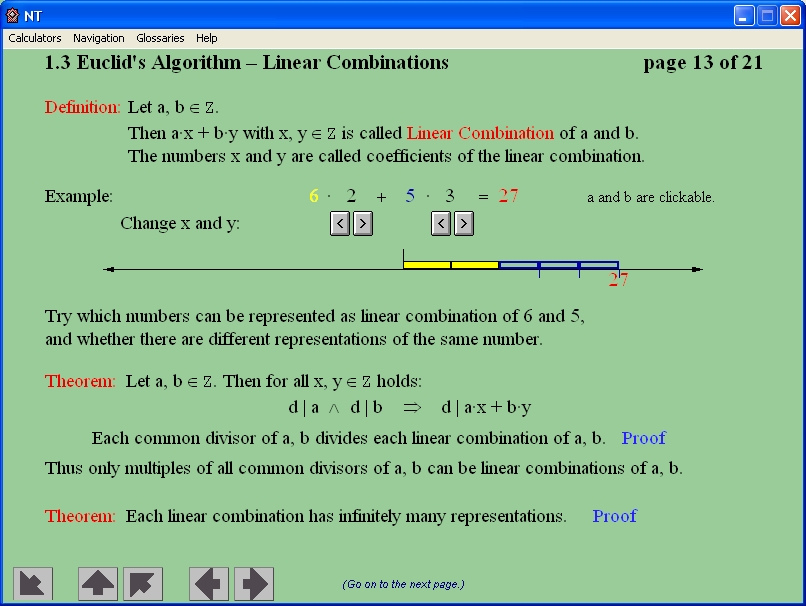
\includegraphics[scale=0.4]{figures/NT_Fig_C1-3_EuclidsAlg-LinearCombinations.png}
\caption{Each common divisor of two integers also divides all its linear
combinations\vspace{1ex}} 
\label{NT_Fig_C1.3_EuclidsAlg-LinearCombinations}
\end{center}
\end{figure}


\begin{figure}[ht]
\begin{center}
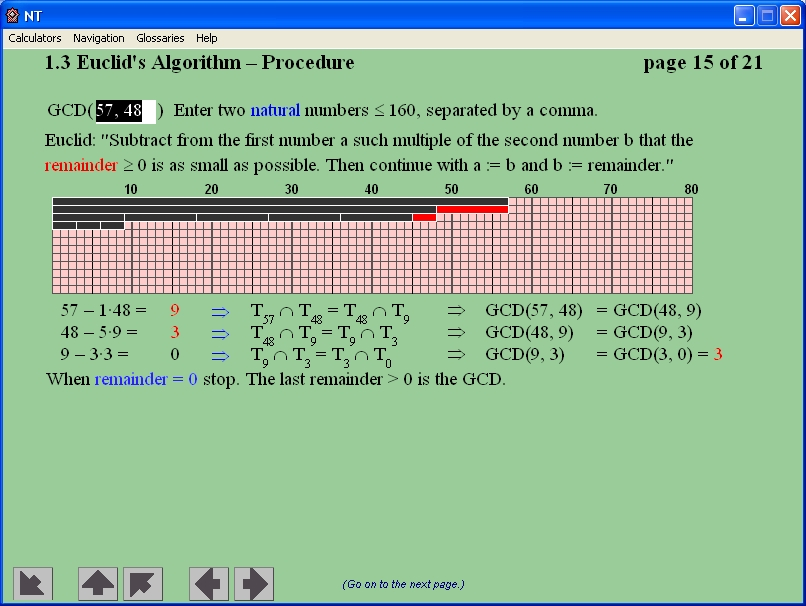
\includegraphics[scale=0.4]{figures/NT_Fig_C1-3_EuclidsAlg-Procedure}
\caption{Euklid's algorithm to determine gcd\vspace{1ex}} 
\label{NT_Fig_C1.3_EuclidsAlg-Procedure}
\end{center}
\end{figure}


\begin{figure}[ht]
\begin{center}
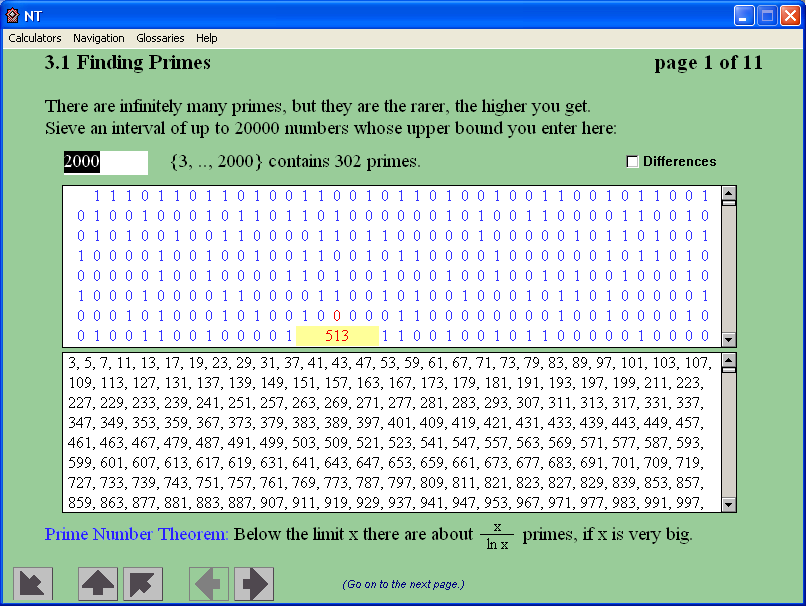
\includegraphics[scale=0.4]{figures/NT_Fig_C3-1_PrimesDistribution}
\caption{Distribution of primes and its differences\vspace{1ex}} 
\label{NT_Fig_C3.1_PrimesDistribution}
\end{center}
\end{figure}


\begin{figure}[ht]
\begin{center}
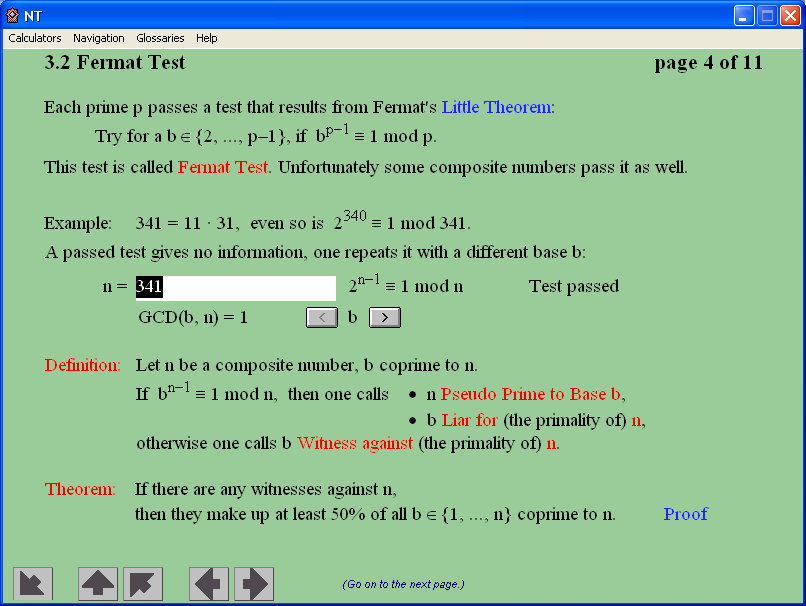
\includegraphics[scale=0.4]{figures/NT_Fig_C3-2_Fermat-Test}
\caption{Finding primes with the prime number test of Fermat\vspace{1ex}} 
\label{NT_Fig_C3.2_Fermat-Test}
\end{center}
\end{figure}


\begin{figure}[ht]
\begin{center}
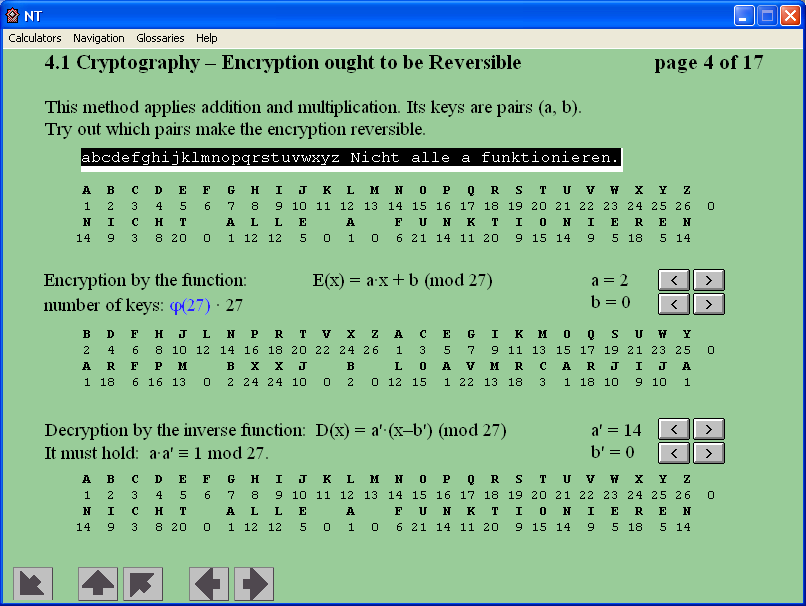
\includegraphics[scale=0.4]{figures/NT_Fig_C4-1_ReversibilityAdditiveCipher}
\caption{Reversibility of encryption mechanisms exemplified with additive
ciphers\vspace{1ex}} 
\label{NT_Fig_C4.1_ReversibilityAdditiveCipher}
\end{center}
\end{figure}


\begin{figure}[ht]
\begin{center}
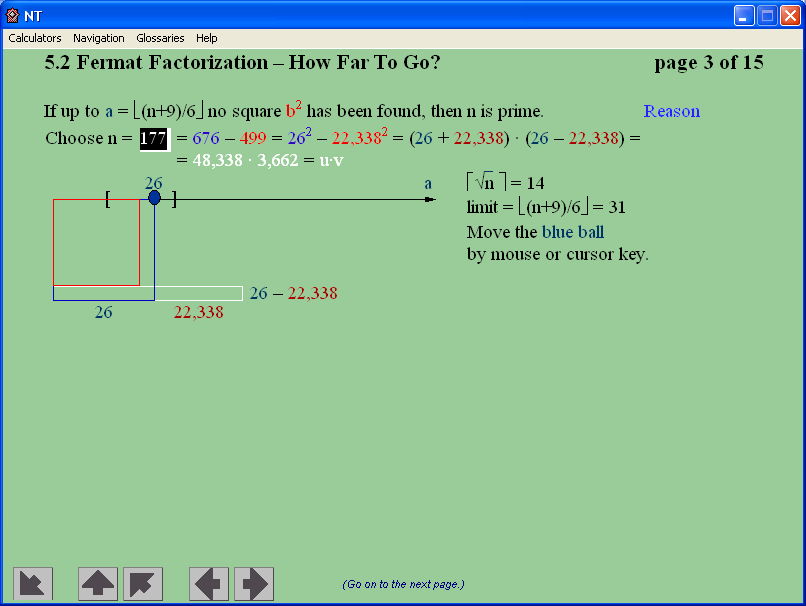
\includegraphics[scale=0.4]{figures/NT_Fig_C5-2_Fermat-factorization-How-far-1}
\caption{Fermat factorization using the third binomial formula\vspace{1ex}} 
\label{NT_Fig_C5.2_Fermat-factorization-How-far-1}
\end{center}
\end{figure}


\begin{figure}[ht]
\begin{center}
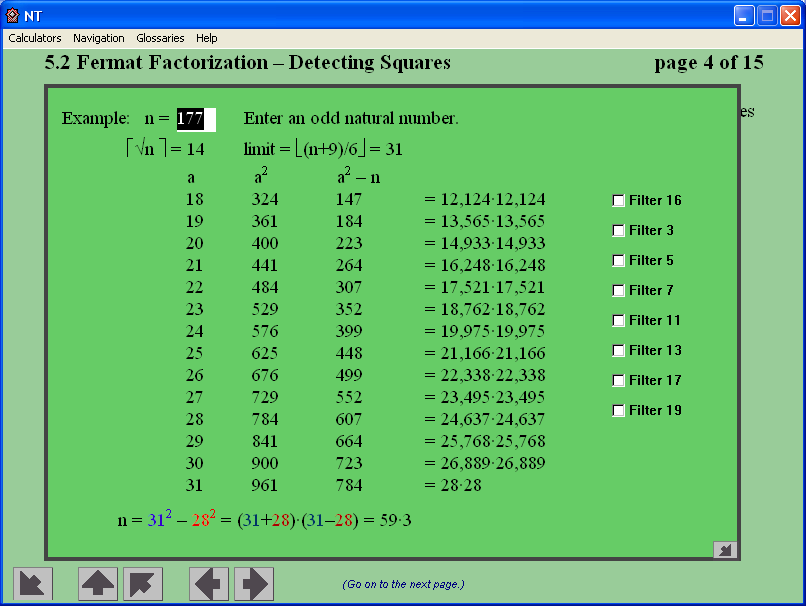
\includegraphics[scale=0.4]{figures/NT_Fig_C5-2_Fermat-factorization-How-far-2}
\caption{Fermat factorization: Detecting squares\vspace{1ex}} 
\label{NT_Fig_C5.2_Fermat-factorization-How-far-2}
\end{center}
\end{figure}


\begin{figure}[ht]
\begin{center}
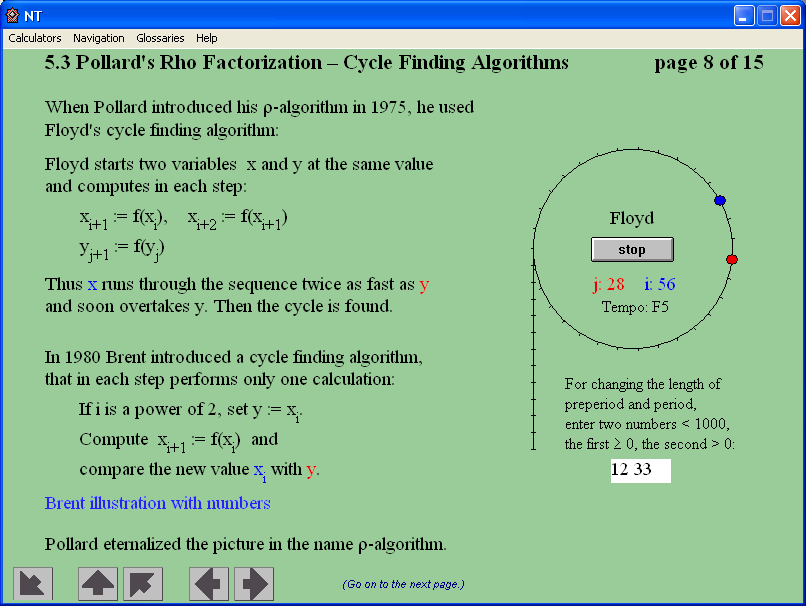
\includegraphics[scale=0.4]{figures/NT_Fig_C5-3_PollardRho}
\caption{Pollard's rho factorization: Floyd's cycle finding algorithm\vspace{1ex}} 
\label{NT_Fig_C5.3_PollardRho}
\end{center}
\end{figure}



% ++++++++++++++++++++++++++++++++++++++++++++++++++++++++++++++++++++++++++
\clearpage
%\newpage
\begin{thebibliography}{99999}
%\addcontentsline{toc}{subsection}{Literaturverzeichnis}

\bibitem[Buchmann2004]{a:Buchmann2004} \index{Buchmann 2004}
    Johannes Buchmann, \\
    {\em Introduction to Cryptography}, Springer, 2nd edition, 2004.

\bibitem[Scheid2003]{a:Scheid2003} \index{Scheid 2003}
    Harald Scheid, \\
    {\em Zahlentheorie}, Spektrum Akademischer Verlag, 3rd edition, 2003.

\end{thebibliography}

